In this chapter, we delve into the analysis and results of our study on gender disparities in match recommendations on the online dating platform Bumble. The primary focus of this investigation is to assess whether the algorithms that drive match recommendations perpetuate gender biases, particularly discriminating against non-binary users compared to their binary counterparts. The importance of this analysis stems from the broader implications of algorithmic bias in social and dating platforms, which can influence societal perceptions and individual experiences in significant ways.

Our research was motivated by the observation that while dating apps have become a ubiquitous medium for interpersonal connections, they also reflect and potentially amplify existing societal biases. This study aims to scrutinize the gender distribution in the match recommendations provided by Bumble, examining the disparities that arise in the treatment of male, female, and non-binary profiles. By investigating these patterns, we aim to uncover any inherent biases encoded in the algorithm's behavior, which could impact the fairness and inclusivity of the dating app.

The methodology adopted for this study involved recruiting participants from diverse gender identities to create profiles on Bumble and monitor the gender of the profiles recommended to them by the platform. This setup allowed us to gather real-world data on how the algorithm curates match recommendations based on user gender, with a special focus on any discrepancies that might disadvantage non-binary users.

By analyzing this data, this chapter seeks to provide a comprehensive understanding of how gender biases may manifest in algorithm-driven match recommendations. Through statistical analysis and qualitative insights, we aim to offer a detailed account of the algorithm’s performance, evaluating its implications for equity and fairness in digital dating spaces.

This analysis is crucial not only for highlighting current issues in algorithmic design but also for guiding future improvements to ensure that dating apps like Bumble promote inclusivity and fairness across all user demographics. By grounding our findings in the broader discourse on algorithmic fairness, this chapter contributes to a more nuanced understanding of the challenges and opportunities in designing equitable digital platforms.

\section{Data Description}
\subsection{Participant Recruitment and Profile Setup}
The dataset for this study consists of data collected from Bumble, specifically focusing on interactions and match recommendations received by the participants. We recruited five participants: two self-identified men, two self-identified women, and one self-identified non-binary person, who were either active or past users of Bumble. This participant selection was strategic, aiming to capture a diverse array of experiences and perspectives, particularly from non-binary individuals, which are often underrepresented in such studies.

Each participant was asked to create two Bumble profiles—one reflecting their self-identified gender and another as their non-binary counterpart. This method was employed to specifically isolate and examine the influence of gender identity on the algorithm’s match recommendations. Both profiles were identical in all respects except the gender designation, ensuring that any observed differences in the data could directly be attributed to the gender variable. This dual-profile approach draws on methodologies used in prior research that investigated user behaviors on digital platforms by manipulating profile characteristics.

\subsection{Data Collection Methodology}
The participants engaged with the app by swiping on other profiles, from which we collected extensive data. This included demographic and personal information such as 
\begin{itemize}
    \item Age
    \item Gender
    \item Work
    \item Education
    \item Location
    \item Hometown
    \item Height 
    \item Activity Level
    \item Star Sign
    \item Drinking Preferences
    \item Smoking Preferences
    \item Kids Preferences 
    \item Relationship preferences
\end{itemize}

These factors are known to influence user interactions and algorithmic recommendations on dating platforms \cite{Tyson_Perta_Haddadi_Seto_2016}. The comprehensiveness of this data collection allowed for a robust analysis of the profiles shown to participants, ensuring a rich dataset for subsequent statistical examination.

\subsection{Data Normalization and Processing}
During the data normalization process, we adjusted the counts of profiles by gender observed by each participant by the total number of profiles they reviewed to ensure comparability across different user interactions. This normalization allowed us to analyze the gender distribution effectively without the skew caused by variable user activity or algorithmic output differences. Additionally, we standardized demographic and behavioral data, such as age groups, education levels, and locations, by categorizing them into broader segments. This standardization facilitated a generalized analysis across a more comprehensive set of user categories, enabling a uniform approach to understanding trends and patterns in the matchmaking algorithm’s behavior.


\section{Analytical Methods}
This section outlines the statistical and computational approaches employed to analyze the data collected from Bumble’s match recommendations. Central to our methodology is the use of a gender-sexuality compatibility matrix, developed specifically for this study to assess how gender identity influences match recommendations. Additionally, we conducted an analysis of demographic parity to compare how the platform's algorithms treat binary and non-binary counterparts.

\begin{figure}[t!]
 \centering
 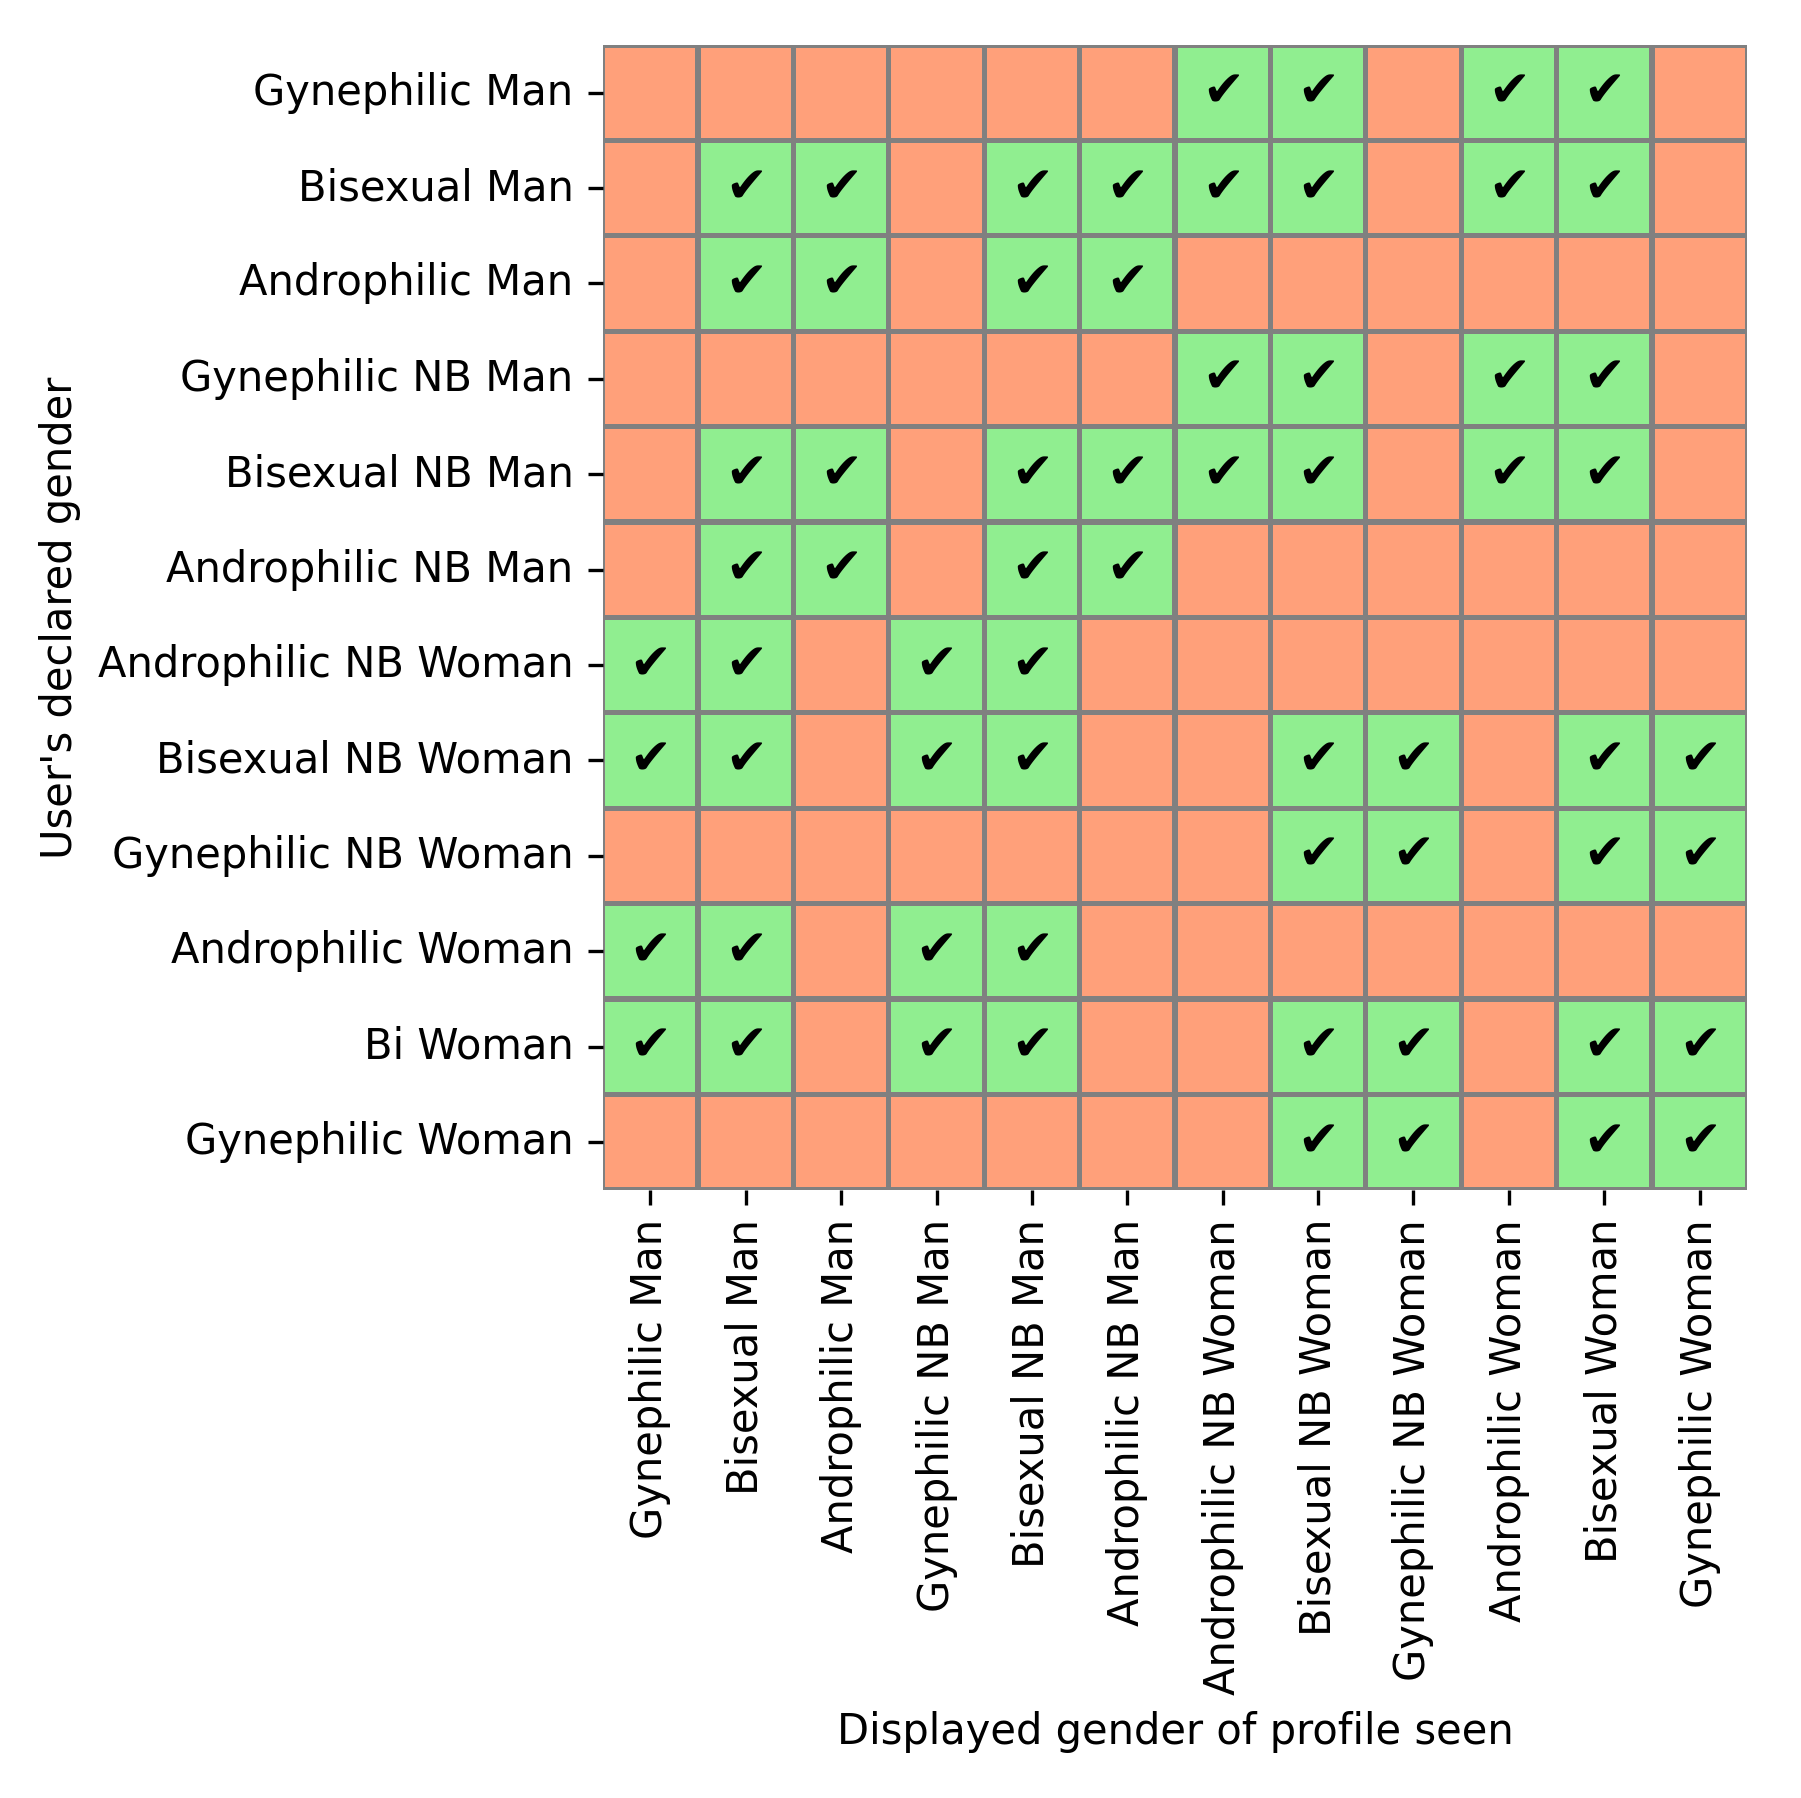
\includegraphics[scale=0.2]{figures/Analysis and Results/gender_matrix.png}
 \caption{Genders-Sexuality Compatibility Grid}
 \label{fig:img3}
\end{figure}

\subsection{Gender Sexuality Comptibility Grid}
The Genders-Sexuality Compatibility Grid Figure \ref{fig:img3} is a atrix const ructed to depict the potential attraction patterns among diverse gender identities and sexual orientations. It systematically represents the interactions between individuals identifying as gynephilic (attracted to women), androphilic (attracted to men), bisexual, across male, non-binary (NB), and female spectrums. Green checkmarks (\checkmark) in the grid signify mutual attraction or compatibility, while red backgrounds indicate incompatibility or lack of attraction.

The development of this grid is grounded in empirical data derived from interviews, and corroborated by analyses of scholarly articles and research papers that explore gender identity and sexual orientation. For instance, studies on childhood gendered behavior and adult sexual attraction patterns provide evidence of the diversity in attraction preferences among androphilic and gynephilic individuals \cite{Petterson_Wrightson_Vasey_2017}.

Research into the sexual attraction of Samoan cisgender and transgender individuals to men and women reveals the intricate cultural expressions of male androphilia, demonstrating the grid's relevance across different cultures \cite{Petterson_Wrightson_Vasey_2017}. The construct of ambiphilia or bisexuality is further substantiated through implicit cognition studies, confirming attraction to both genders \cite{Snowden_Fitton_McKinnon_Gray_2020}.

Moreover, evolutionary perspectives on male androphilia elucidate the shared biological and developmental correlates underlying this sexual orientation, informing the structure of the grid \cite{Vasey_VanderLaan_2014}. These insights confirm that, despite differences in cultural gender roles, sexual attraction follows consistent patterns.

Using this matrix, we were able to systematically track and analyze the distribution and frequency of match recommendations across different gender pairings. This method allowed us to discern patterns or biases in how the algorithm recommends profiles, which is crucial for understanding the extent to which Bumble’s algorithm might perpetuate existing societal biases.

\subsection{Verification of Demographic Parity}
To assess fairness in algorithmic recommendations, we employed the concept of demographic parity. This involves comparing the match recommendations received by binary gender users (men and women) with those received by their non-binary counterparts. When setting your gender as Non-Binary on Bumble, it asks you to fill in which gender categroy you want your profile to show as, i.e., either Man or Woman. So for the purpose of this study, we define the non-binary counterparts as follows:

\begin{itemize}
    \item \textbf{Non-Binary Man:} A profile set up by a participant with Non-Binary as gender, and 'Appear in Searches' as Man.
    \item \textbf{Non-Binary Woman:} A profile set up by a participant with Non-Binary as gender, and 'Appear in Searches' as Woman.
\end{itemize}

These definitions align with the operationalization of gender in our dataset, ensuring that the comparisons we make are grounded in the lived experiences of non-binary individuals using Bumble.

By verifying demographic parity, we aimed to discover whether the algorithm shows a preference for certain genders, thereby disadvantaging others. This analysis involved comparing the rates at which different genders were shown to man vs. non-binary man and woman vs. non-binary woman profiles. It is a crucial step in determining whether the matching algorithm enforces or mitigates gender bias, thereby influencing the inclusivity and fairness of the platform.

\subsection{Statistical Techniques}
The primary statistical technique employed in this analysis was the Chi-squared test of independence. This test was used to examine the relationship between the gender identity of the profile user (man, non-binary man, woman, non-binary woman) and the gender identity of the profiles they were shown by Bumble's matching algorithm. The Chi-squared test is particularly useful for categorical data analysis, as it helps determine whether there is a statistically significant association between two categorical variables.

For this study, the Chi-squared test allowed us to assess the null hypothesis that gender identity of the user does not influence the gender of the profiles shown to them. This hypothesis was tested across different gender pairings within the data, such as man versus non-binary man and woman versus non-binary woman, to identify any disparities in how different genders were treated by the algorithm.

The result of the Chi-squared test yielded a p-value of 0.039, indicating that there are statistically significant differences in the distribution of gender in match recommendations based on the user’s gender identity. This finding suggests that the algorithm may be influencing match recommendations in a way that does not equally represent gender identities, thus potentially contributing to a bias in how users are paired on the platform.

This statistical evidence forms a critical part of the analysis, as it provides a quantitative basis for discussing algorithmic fairness and the representation of gender diversity in Bumble's match recommendations.

\section{Profile Analysis Results}
The results of our analysis highlight significant findings regarding the gender distribution in match recommendations provided by Bumble. The primary attribute analyzed was the gender of profiles recommended to users of different gender identities. We quantified the profiles by gender for each user, normalized these counts against the total number of profiles displayed, and calculated the mean for users of each declared gender. This methodological approach enabled a rigorous evaluation of the distribution of profiles across genders, offering a systematic understanding of how the algorithm mediates match recommendations based on user gender.

\begin{figure}[t!]
 \centering
 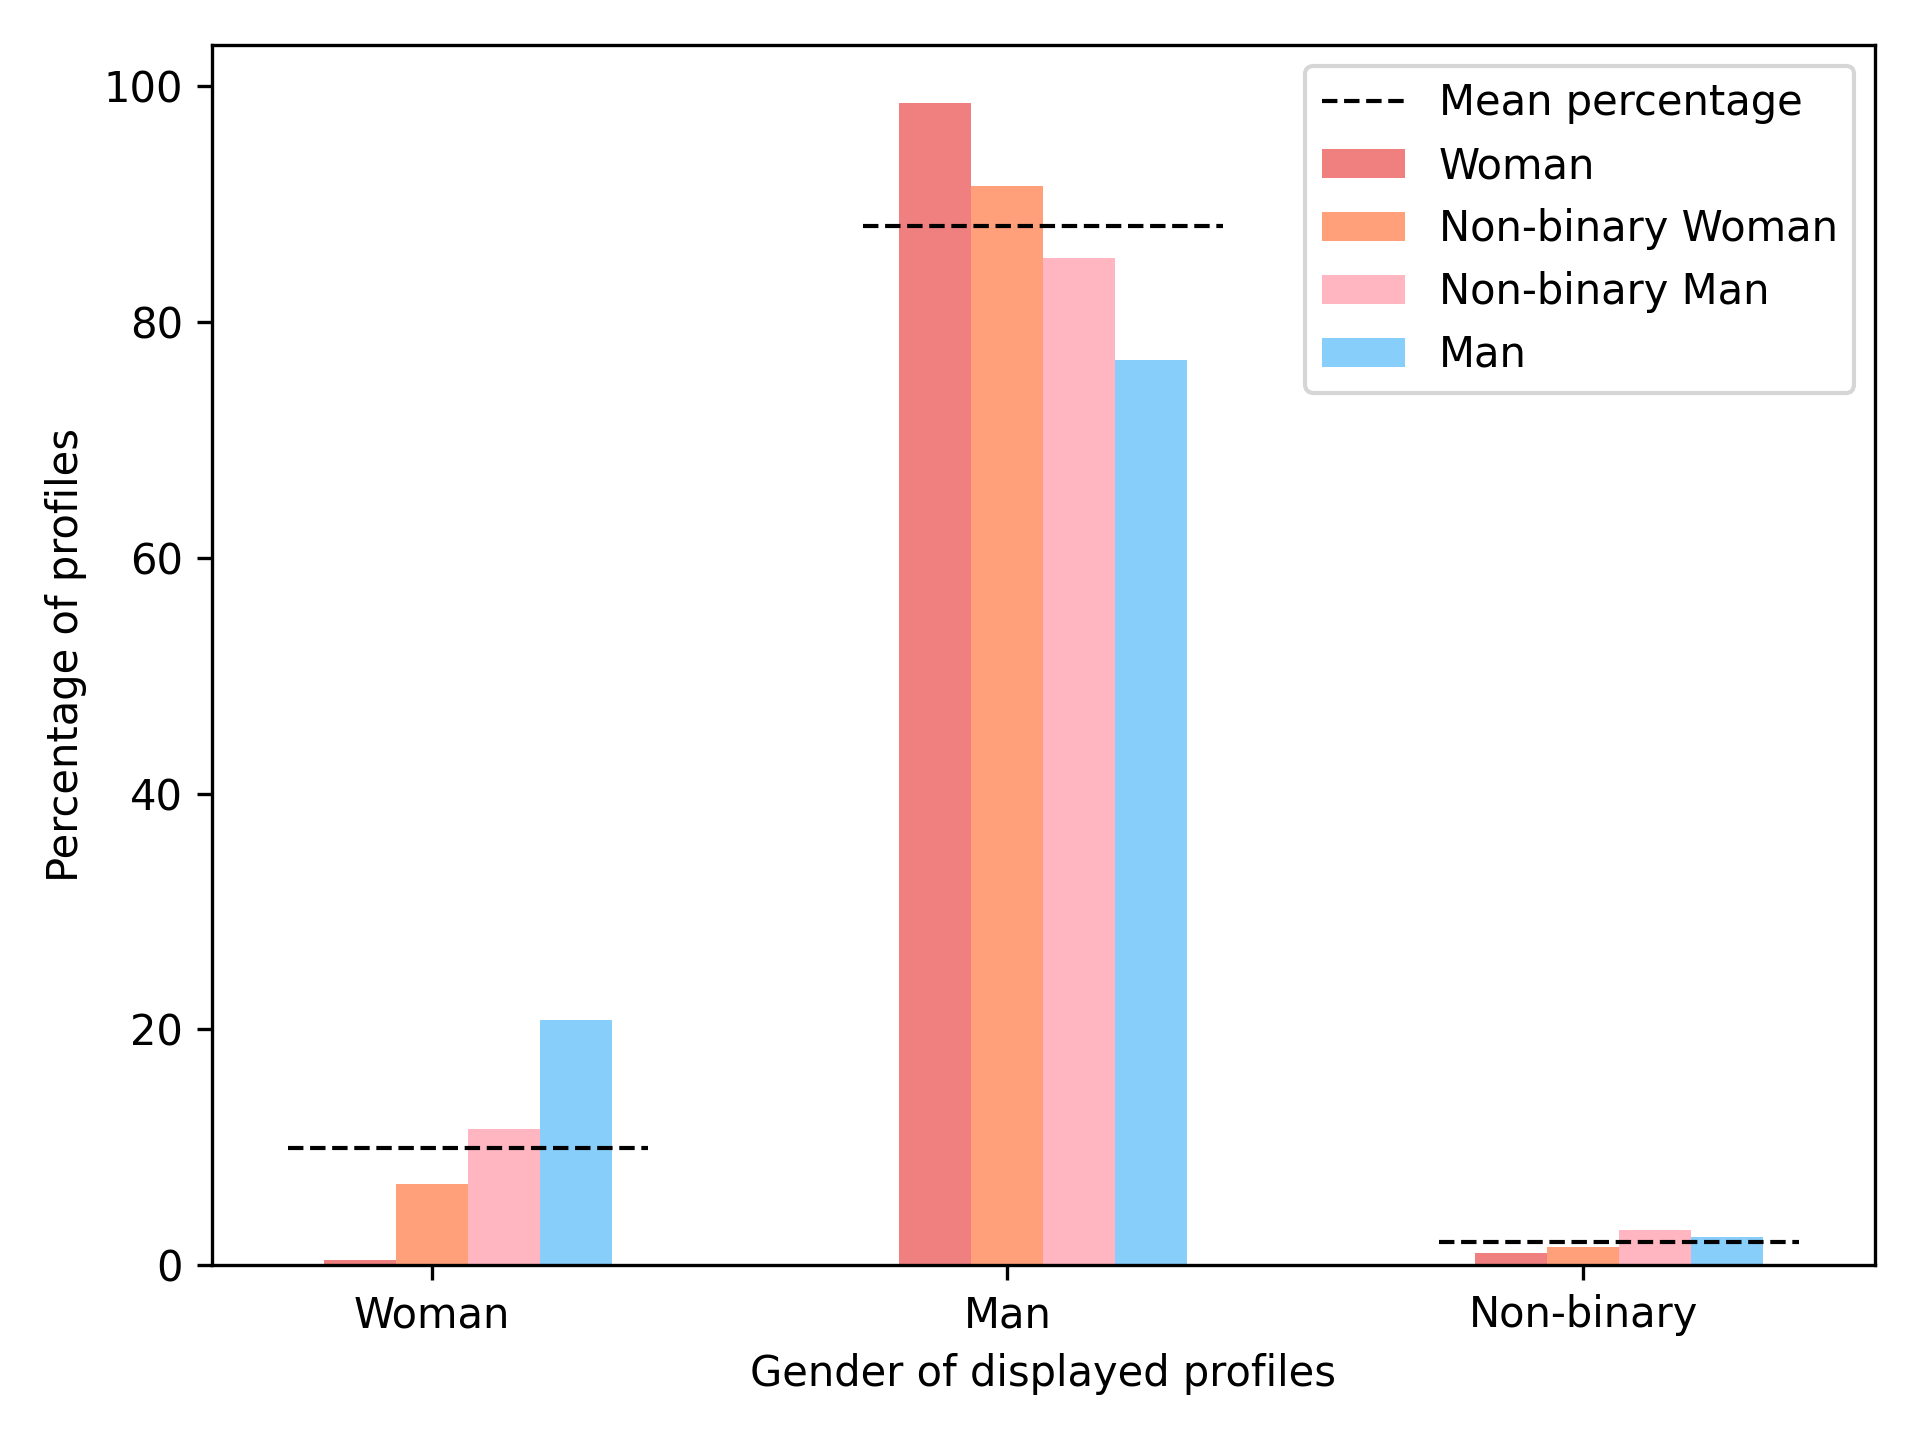
\includegraphics[scale=0.8]{figures/Analysis and Results/gender_percentage.png}
 \caption{Percentage of Genders displayed in our Profiles}
 \label{fig:img4}
\end{figure}

Our analysis revealed discernible skews in the gender distribution of match recommendations. Notably, for our male profiles, the number of female profiles displayed was 9.1\% higher compared to their non-binary male counterparts. Conversely, female profiles experienced a 6.8\% higher exposure to male profiles than did their non-binary female counterparts. These disparities suggest a potential bias in the algorithm's recommendation system, where the gender identity of the user appears to influence the gender composition of the profiles shown. This finding is significant as it suggests that Bumble’s algorithm may not treat gender identity neutrally but rather modulates match visibility in a way that could disadvantage non-binary users.

Another significant trend observed in our analysis concerns the skewed distribution between the number of men and women displayed to users. Generally, the proportion of men shown to users is substantially higher. This trend reflects the overall gender ratio among Bumble users, as derived from our dataset, where men constitute 88.12\% of profiles, women make up 9.92\%, and non-binary individuals account for 1.96\%.

This imbalance in gender representation is even more pronounced when comparing the gender ratios of the profiles shown with the gender of the participants themselves. Specifically, our findings show that men are disproportionately shown to women users compared to how often women are shown to men users. This indicates a potential bias in the algorithm’s process of generating match recommendations, which tends to favor the display of male profiles over female or non-binary profiles.

\section{Interviews Analysis}
The qualitative insights derived from interviews conducted with Bumble users, particularly those who identify as bisexual, offer a detailed look into the lived experiences and challenges faced on the dating platform. These interviews shed light on the nuanced ways in which the application’s algorithms impact user experiences, particularly in terms of gender representation and the accuracy of match recommendations. The firsthand accounts reveal not only algorithmic shortcomings but also provide critical user perspectives on the platform's operational dynamics.

\subsection{Key Themes from the Interviews}
\begin{itemize}
    \item \textbf{Discrepancies in Gender Representation:} Interviewees frequently pointed out a significant skew in gender representation, especially noting an overrepresentation of male profiles despite their preferences set for females. This discrepancy is crucial as it reflects a misalignment between user settings and profile recommendations, with one user expressing, "I'm shown more men than women even when I don’t have everyone (filter) on... it's like an epidemic just men marking their profile as women whose preference is women" (Subject A). Another user highlighted, "It's mostly men being shown - it probably is mostly men because like there's a lot of men on profiles yes but also a lot of men were marked as women are probably shown but because you have everyone turn on you don't notice it" (Subject A), and "I just see a lot of men" (Subject C) underscoring the challenges posed by gender misrepresentation.
    \item \textbf{Algorithmic Limitations and Misclassifications:} The issue of men misrepresenting their gender to appear in searches intended for women was a significant concern, particularly affecting lesbian and bisexual women. This misclassification leads to frustration and mistrust in the platform's ability to cater effectively to user preferences, as evidenced by comments from the interviews: "I'll show you something yeah but it's like an epidemic just men marking their profile as women whose preference is women" (Subject A).
    \item \textbf{Impact on User Experience and Preferences:} The frustrations stemming from discrepancies in gender representation and algorithmic misclassification directly diminish user experience and satisfaction. As one user bluntly put it, "I have everyone right now, I don't enjoy using Bumble" (Subject A).
    \item \textbf{Safety and Inclusivity Concerns:} Safety issues emerged as a recurrent theme, with users feeling unsafe due to the misrepresentation of profiles and the absence of robust filters to mitigate such experiences. This is captured in remarks such as, "Also like it feels a little unsafe to just meet a random man from a dating profile as opposed to like uh of a woman" (Subject A), and "I used to see that ('Potential Match Missed' message) at time and that would be after I swiped left on (let's say) a 30-40 year old man and that was creepy for me" (Subject B) and the need for platform improvements: "Fixing the men marking themselves as women thing definitely would be like a very major thing because it's literally like taking you off the app" (Interview 5).
    \item \textbf{Potential for Algorithmic Improvement:} Users suggested several improvements to enhance the algorithm, such as better filtering options and the capability to have separate feeds for different genders, which could significantly enhance user experience. These suggestions are encapsulated in statements like, "If it like um showed you not like equally but like based on how much you have swiped in the past on women versus men that would probably be a good like balance" (Subject A), and "I think they should have different recommendation algorithms for men and women" (Subject A), indicating a pathway towards more personalized and effective matching processes.
\end{itemize}  

\section{Integration of Quantitative and Qualitative Insights}
The quantitative analysis of profile distributions and the qualitative insights gained from user interviews in this study complement each other, providing a holistic understanding of the gender biases present in Bumble's matchmaking algorithms.

The quantitative analysis involved systematically counting and normalizing the profiles by gender shown to each participant. This data provided a clear, objective measure of how gender influences the profiles that users are shown. By quantifying these distributions, we established a baseline understanding of the gender dynamics within the app. The statistical significance of these findings, evidenced by disparities in gender representation (men being predominantly shown to women and vice versa), underscores potential biases in the algorithm's recommendation system.

On the other hand, the interviews offered nuanced, subjective insights that qualitative data alone could not capture. Participants shared their personal experiences and perceptions regarding the diversity and inclusiveness of the profiles they encountered. These discussions revealed the practical impact of the observed quantitative disparities on user experience. For instance, several female and non-binary participants noted a sense of frustration or exclusion due to the overwhelming number of male profiles, which aligned with the quantitative data showing a higher percentage of male profiles in their match recommendations.

Together, these methods paint a comprehensive picture of the algorithm's behavior and its effects on users. The quantitative data highlights systemic issues and patterns that require attention, while the qualitative insights provide context and depth, illustrating how these patterns affect real people's interactions on the platform. This dual approach not only strengthens the validity of the findings by corroborating quantitative data with real-world experiences but also enriches the discussion on how to improve algorithmic fairness and inclusivity in digital dating spaces.

\section{Discussions}   
